\documentclass[10pt]{article}
\usepackage{amsmath}
\usepackage{graphicx}
\usepackage{mathrsfs}
\usepackage[margin=0.0in]{geometry}
\begin{document}
	Equations:
	
	Generalised Serre - SWWE equations - $\epsilon$ introduced which when $\epsilon =1$ gives Serre and when $\epsilon = 0$ gives SWWE
	
	They are:
	
	\[
	\frac{\partial h}{\partial t} + \frac{\partial (uh)}{\partial x} = 0
	\]
	\[
	\frac{\partial G}{\partial t} + \frac{\partial }{\partial x} \left ( Gu + \frac{gh^2}{2} - \epsilon \frac{2 h^3}{3} \frac{\partial u}{\partial x} \frac{\partial u}{\partial x} \right ) = 0 \]
	where a new conserved quantity, $G$ is given by
	\[
	G = uh - \epsilon \frac{\partial }{\partial x} \left ( \dfrac{h^3}{3} \frac{\partial u}{\partial x} \right ).
	\]
	
	I forced a solution by introducing $h^*$,$u^*$,$G^*$ and solving the forced version of these equations:
	
	\[
	\frac{\partial h}{\partial t} + \frac{\partial (uh)}{\partial x} = \frac{\partial h^*}{\partial t} + \frac{\partial (u^*h^*)}{\partial x}
	\]
	\[
	\frac{\partial G}{\partial t} + \frac{\partial }{\partial x} \left ( Gu + \frac{gh^2}{2} - \epsilon \frac{2 h^3}{3} \frac{\partial u}{\partial x} \frac{\partial u^*}{\partial x} \right ) = \frac{\partial G^*}{\partial t} + \frac{\partial }{\partial x} \left ( G^*u^* + \frac{g(h^*)^2}{2} - \epsilon \frac{2 (h^*)^3}{3} \frac{\partial u^*}{\partial x} \frac{\partial u^*}{\partial x} \right ) \]
	
	where RHS is calculated analytically and LHS is approximated numerically using $\text{FDVM}_2$ (second-order finite difference volume method)
	
	I used 
	\[h^* = a_0 + a_1 \exp \left[ \dfrac{\left(x - a_2 t\right)^2}{2a_3}\right]\]
	\[u^* = a_4 \exp \left[ \dfrac{\left(x - a_2 t\right)^2}{2a_3}\right]\]
	\[
	G^* = u^*h^* - \epsilon \frac{\partial }{\partial x} \left ( \dfrac{(h^*)^3}{3} \frac{\partial u^*}{\partial x} \right ).
	\]
	
	With
	$x \in \left[-50,100\right]$\\
	Number of cells varied like so $n = 100\times2^k$ with $k \in \left[0,9\right]$\\
	$$\Delta x = \frac{100 - (-50)}{n}$$
	$$\frac{\Delta t}{\Delta x} = \frac{Cr}{a_2 + a_4 + \sqrt{g(a_0 + a_1)}}$$
	$Cr = 0.5$, 
	$g =   9.81 $,  
	$a0 =   1.0$,   
	$a1 =   1.0$,   
	$a2 =   5.0$,    
	$a3 =   10.0$,    
	$a4 =   1.0$
	
	Results:
	 
	I have plotted results for various $\epsilon$ values together to demonstrate method can handle both extremes (SWWE and Serre) as well as inbetween values.
	
	Example Solutions

	\begin{figure}[h!]
		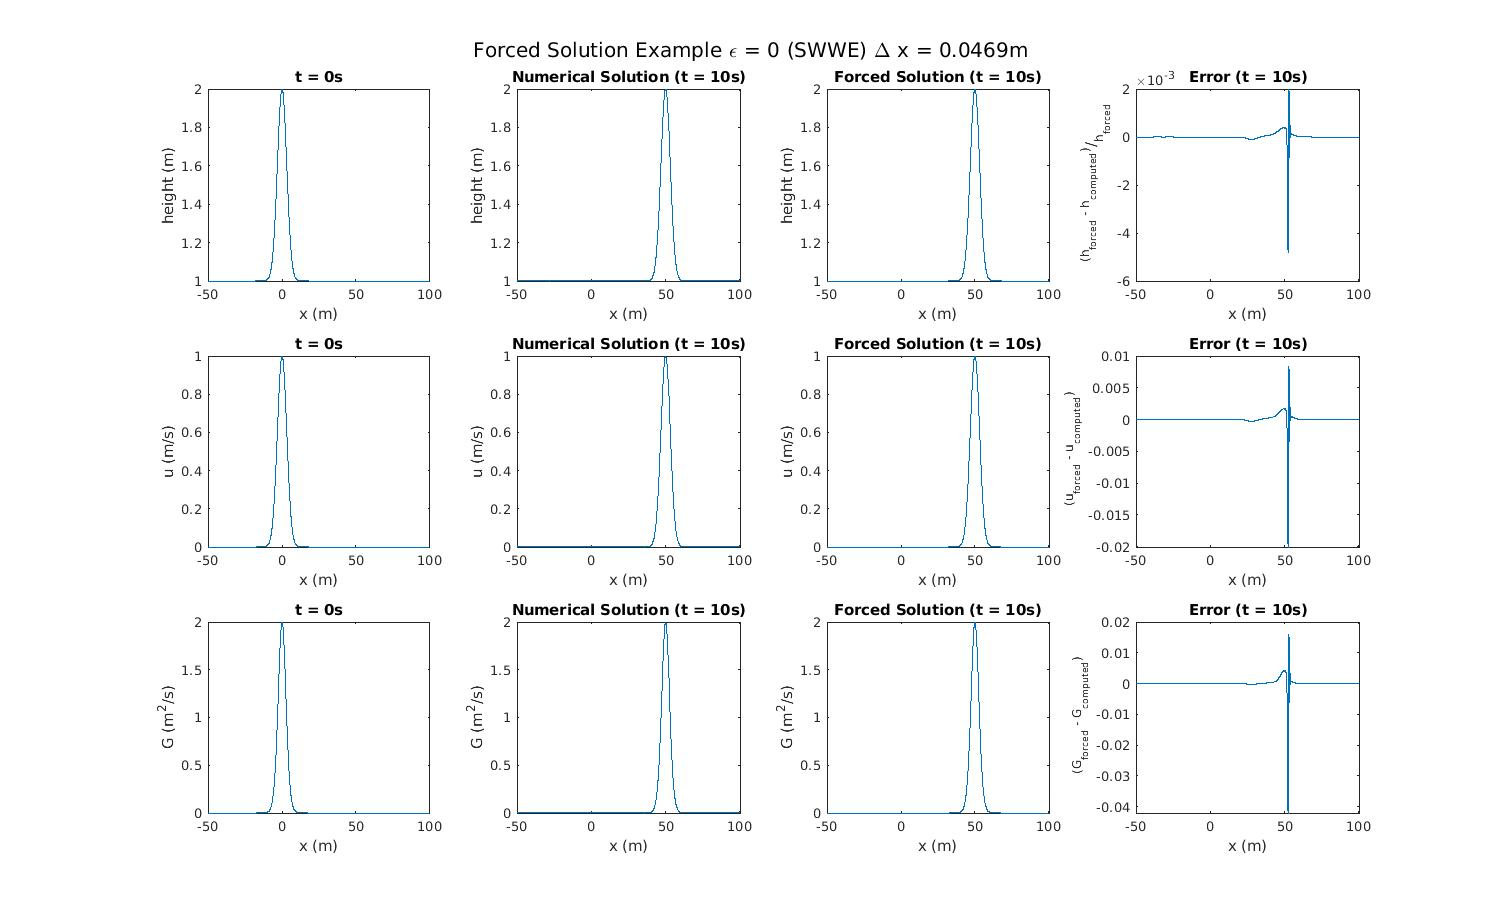
\includegraphics[width=23.0cm]{ExampleEps0.jpg}
		\caption{$\epsilon = 0$ (SWWE)}
	\end{figure}

	\begin{figure}[h!]
	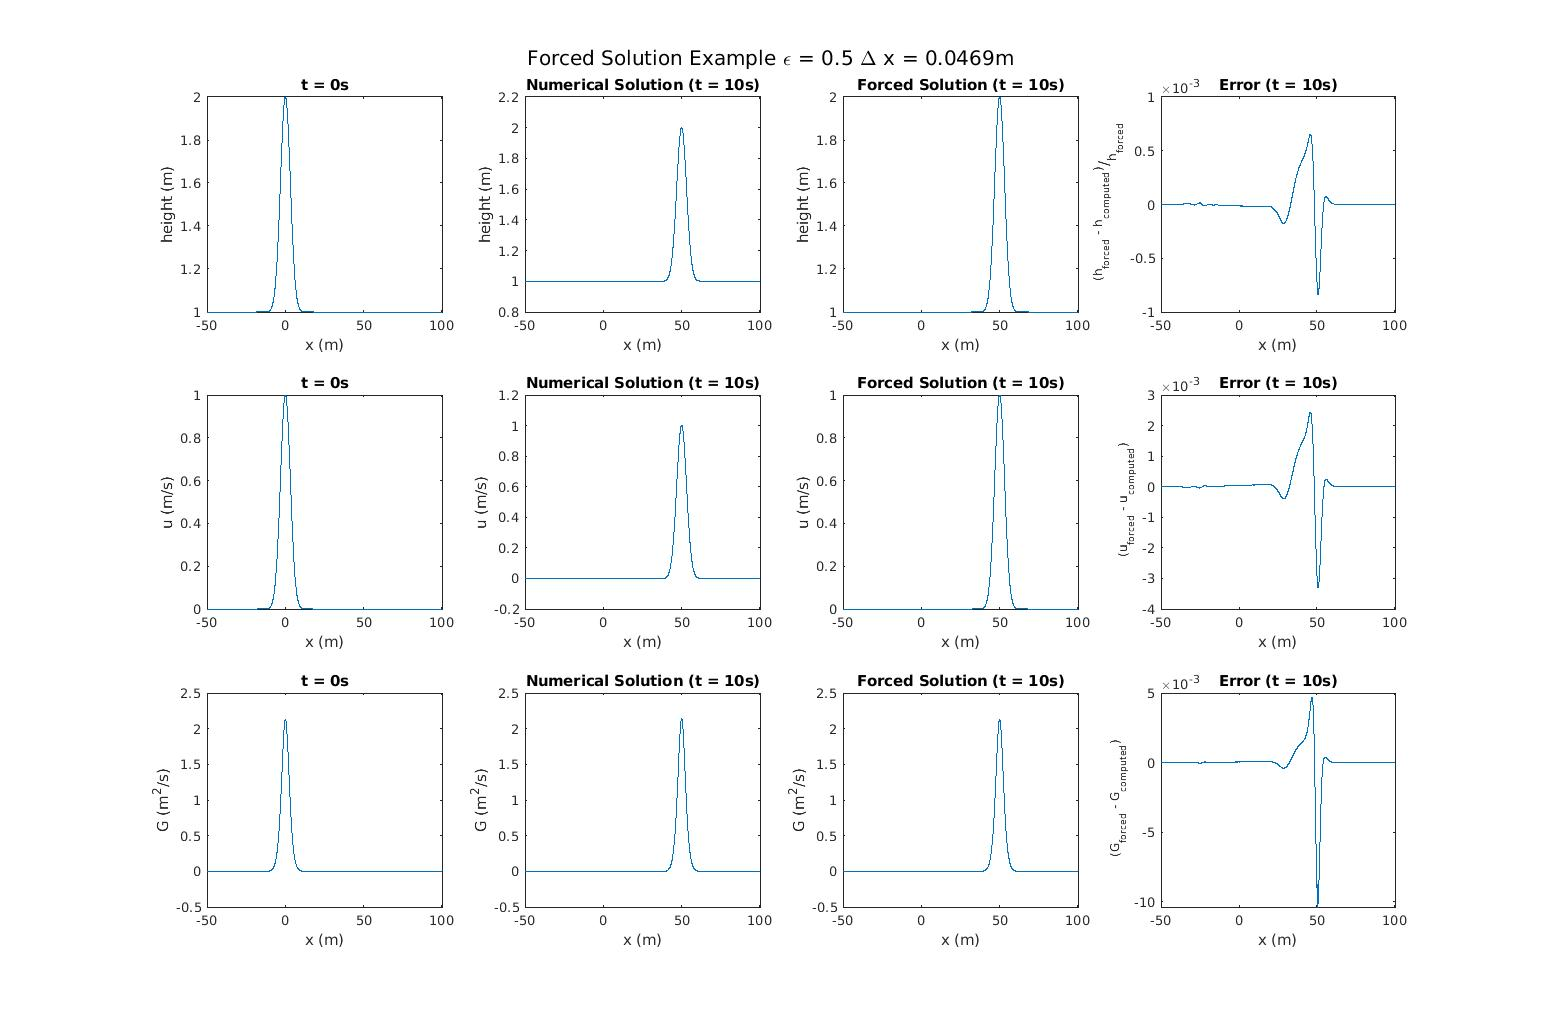
\includegraphics[width=23.0cm]{ExampleEps0p5.jpg}
	\caption{$\epsilon = 0.5$ }
	\end{figure}

	\begin{figure}[h!]
	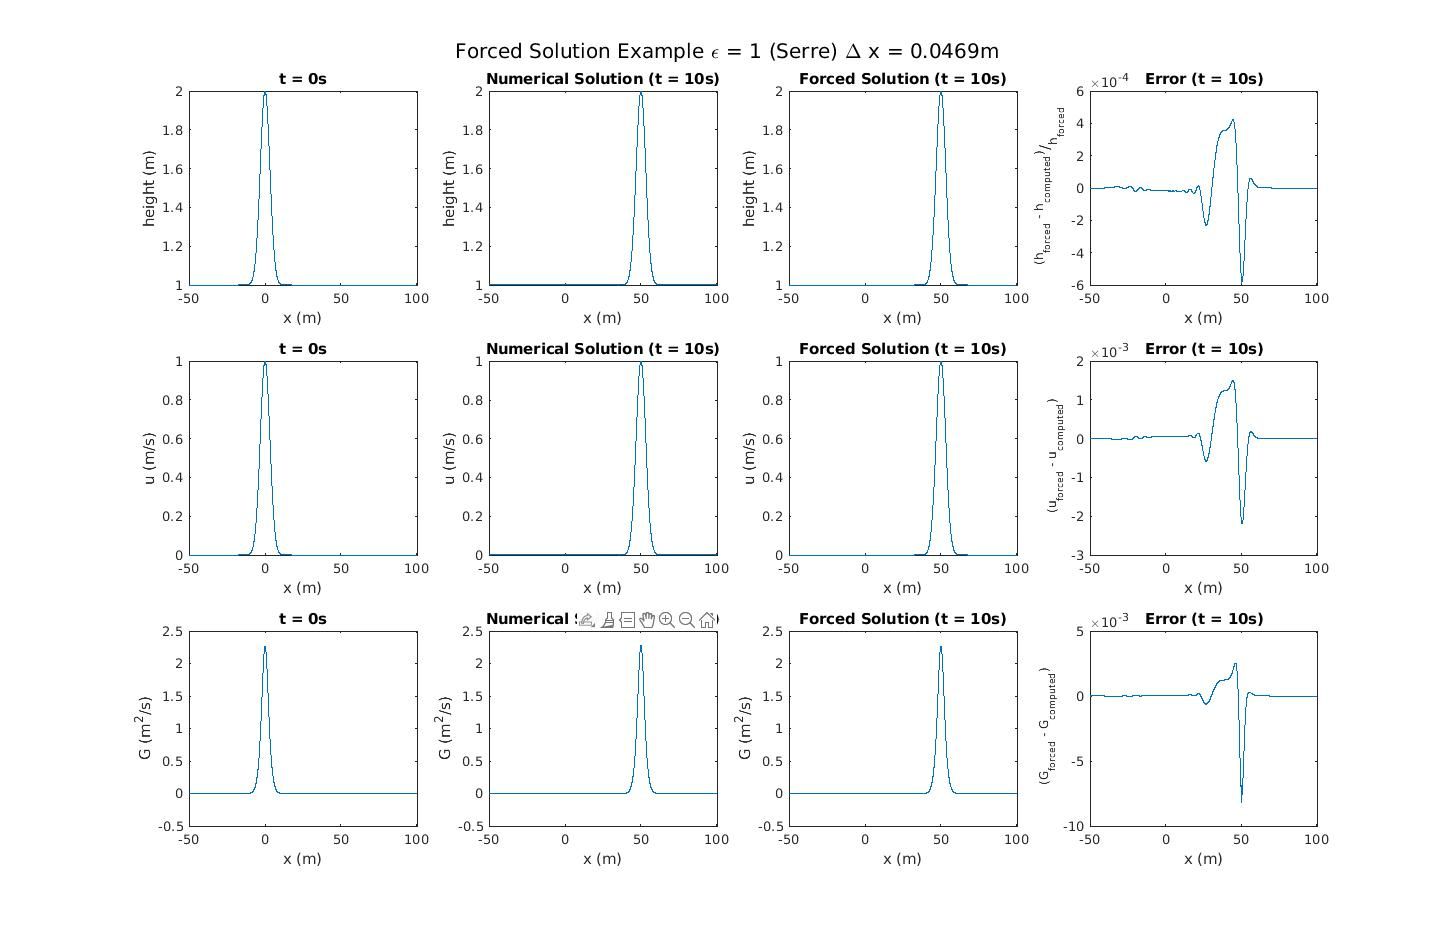
\includegraphics[width=23.0cm]{ExampleEps1.jpg}
	\caption{$\epsilon = 1$ (Serre)}
	\end{figure}
	
	Convergence with second order slope shown
	
	\begin{figure}[h!]
		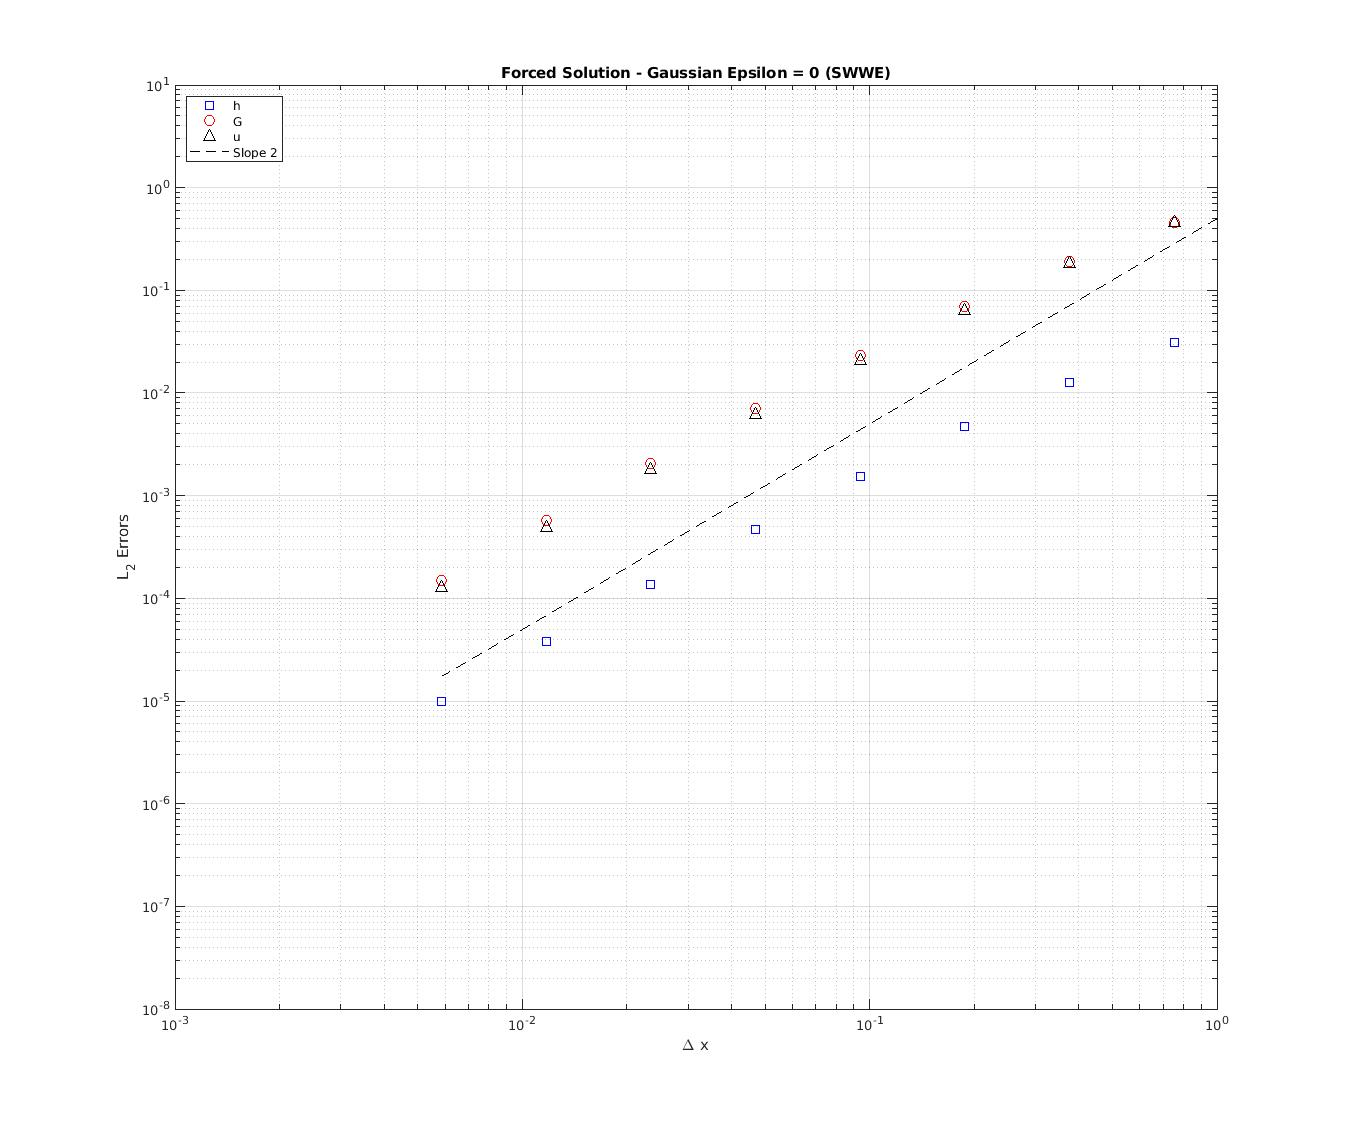
\includegraphics[width=23.0cm]{L2NormsEps0.jpg}
		\caption{$\epsilon = 0$ (SWWE)}
	\end{figure}
	
	\begin{figure}[h!]
		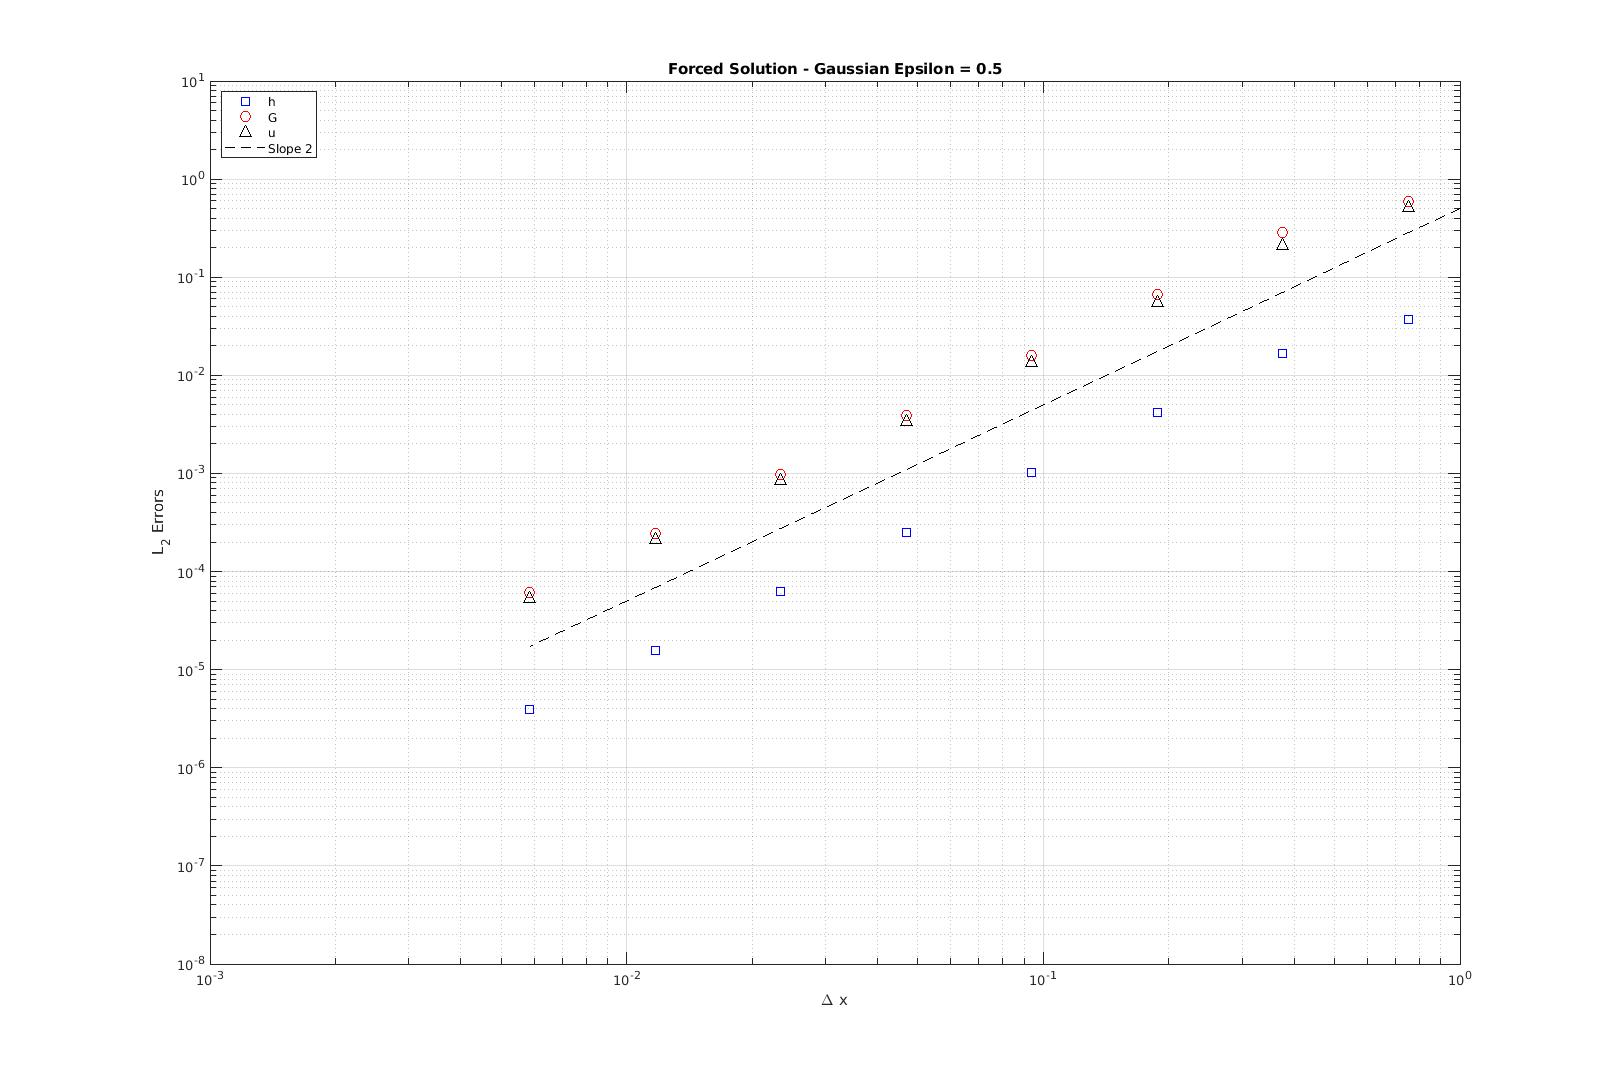
\includegraphics[width=23.0cm]{L2NormsEps0p5.jpg}
		\caption{$\epsilon = 0.5$ }
	\end{figure}
	
	\begin{figure}[h!]
		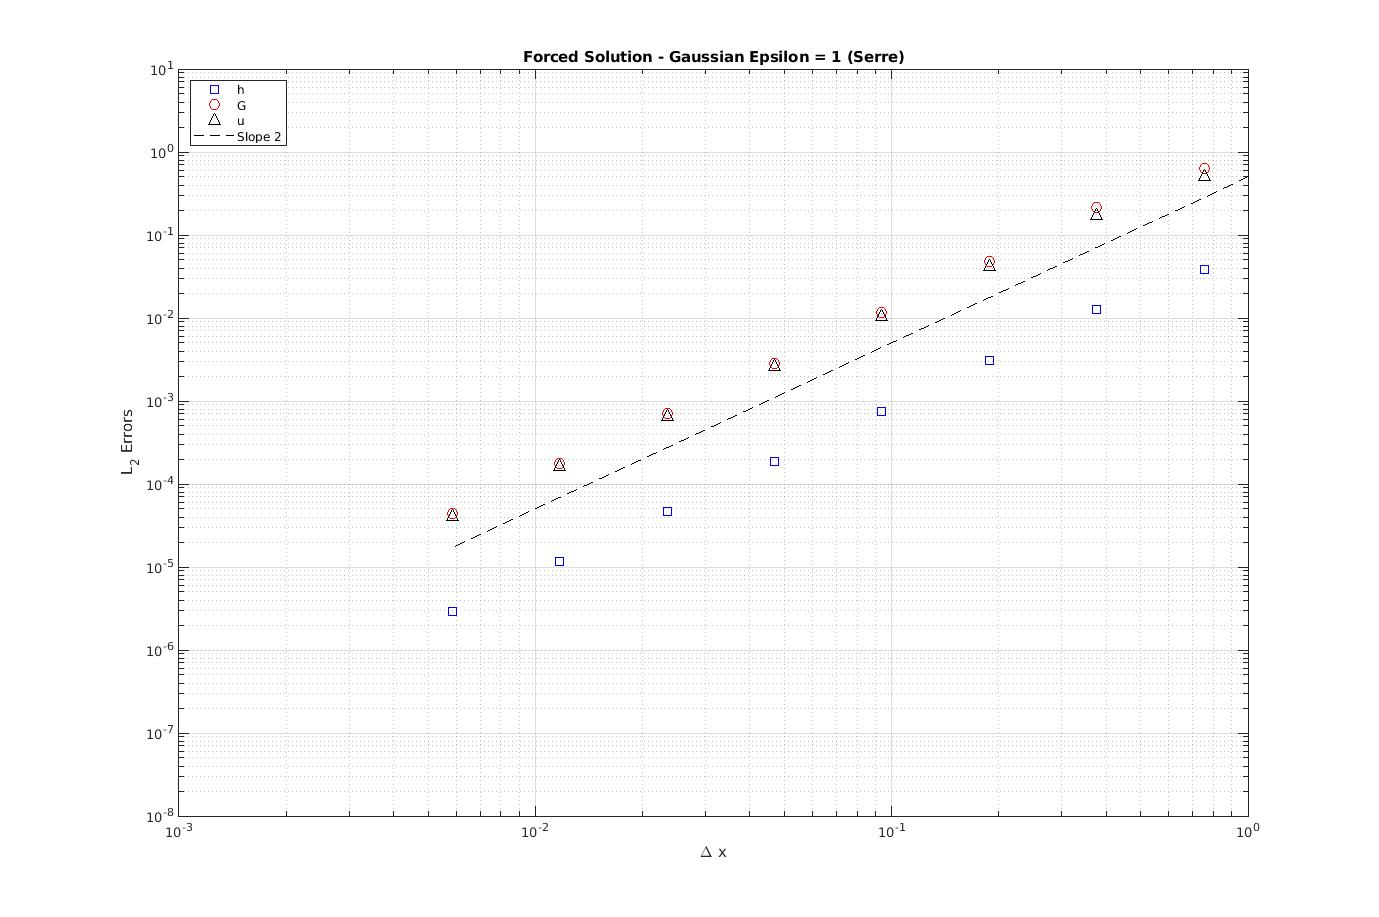
\includegraphics[width=23.0cm]{L2NormsEps1.jpg}
		\caption{$\epsilon = 1$ (Serre)}
	\end{figure}
	  
\end{document}